\section{Experiments}
\label{sec:experiments}

\subsection{Head-only adaptation}
\label{sec:exp:head}
Head-only training was run per dataset family and evaluated on the deployed
map, not on validation pairs. Deployed LPIPS improves on four of five
families: ETH3D $-29.1\%$, EuRoC $-20.8\%$, TUM $-7.9\%$ to $-25.9\%$ over
four sequences, Replica positive, and 7-Scenes the weak family
($+0.14\%$ to $-4.9\%$). The result is seed-robust: two heads $\times$ two
seeds, checked at both validation and deployment level, gave relative deltas
under $5\%$ with inconsistent signs --- ordinary noise rather than fragility.

\paragraph{Four falsified attributions.}
We attempted to explain why some families gain far more than others, and
failed. \Cref{tab:falsified} lists the candidates: each was pre-registered
with the cell that would refute it, and each was refuted by direct
measurement rather than by argument. We report this as a negative result. The
gains are real --- they exceed a measured $0.17\%$ LPIPS noise floor --- but we
decline to adopt the most plausible surviving story in the absence of an
out-of-sample test.

\begin{table}[t]
\centering\small
\setlength{\tabcolsep}{3pt}
\begin{tabular}{@{}p{0.30\linewidth}p{0.62\linewidth}@{}}
\toprule
Candidate & Why it fails \\
\midrule
Scale-frame consistency &
Mechanically inert: \cref{eq:splatt3rloss} is purely photometric, means are
\texttt{detach()}ed, and the metric-scale flag's only consumer is disabled.
Depth touches training solely via the mask. \\
Supervision coverage &
Measured per family: EuRoC has the \emph{lowest} coverage ($39.5\%$) and the
second-largest gain; ETH3D matches TUM's coverage ($61.9$ vs $60.0\%$) with
$3\times$ the gain. \\
Opacity un-saturation &
Explains four families in rank order but 7-Scenes measures $0.479$ ---
comparable to EuRoC's $0.38$ --- with a null gain. A measured counterexample,
not a pending cell. \\
Base-checkpoint headroom &
$\rho=0.145$ over $11$ sequences. ETH3D \texttt{sofa\_1} has the lowest
deficit of any sequence and the second-largest gain. \\
\bottomrule
\end{tabular}
\caption{Four pre-registered mechanisms for the cross-family variation, each
killed by measurement. The variation is real and remains unattributed.}
\label{tab:falsified}
\end{table}

\begin{figure*}[t]
  \centering
  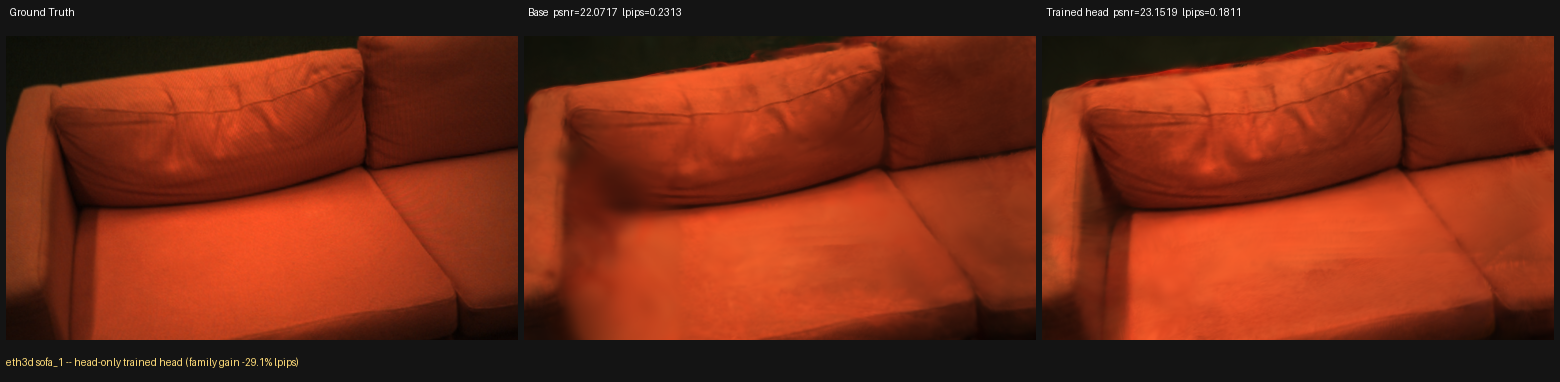
\includegraphics[width=0.92\linewidth]{fig/eth3d_sofa1_f1.png}\\[2pt]
  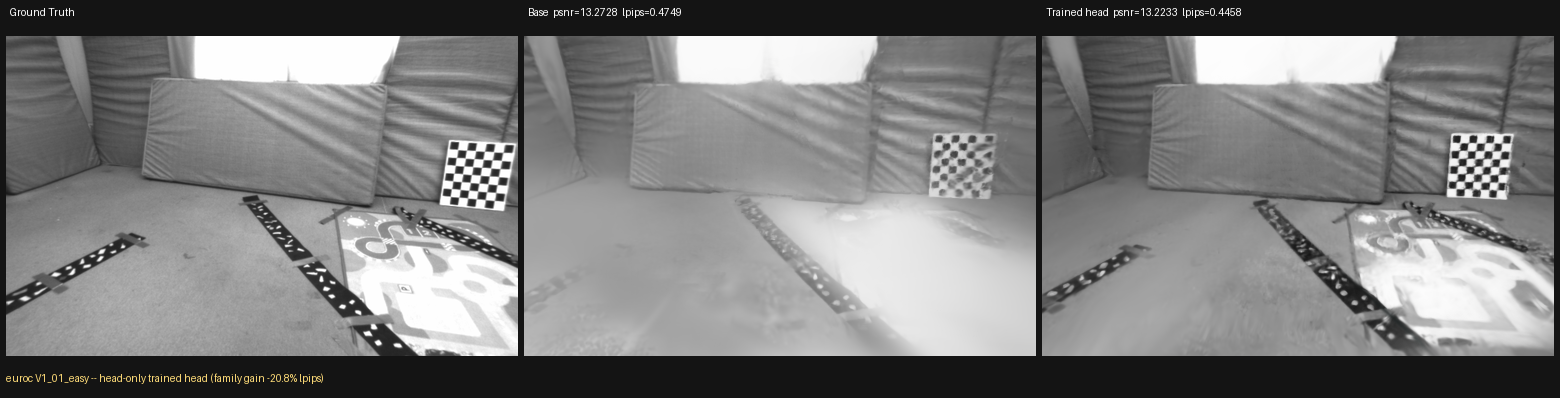
\includegraphics[width=0.92\linewidth]{fig/euroc_v101_f0.png}\\[2pt]
  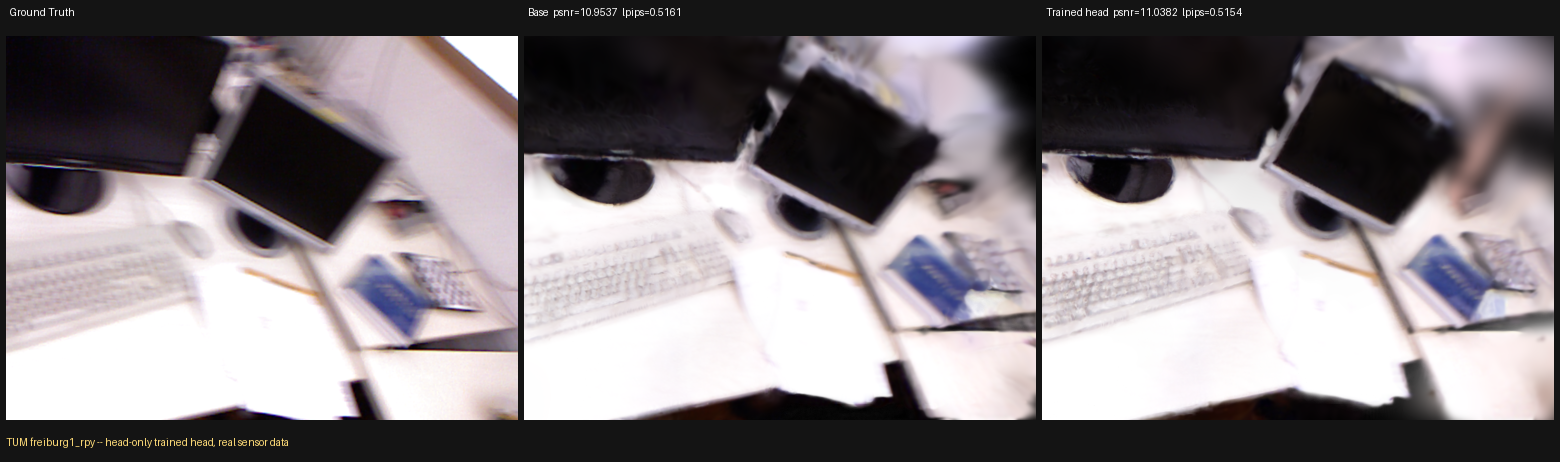
\includegraphics[width=0.92\linewidth]{fig/tum_rpy_f0.png}\\[2pt]
  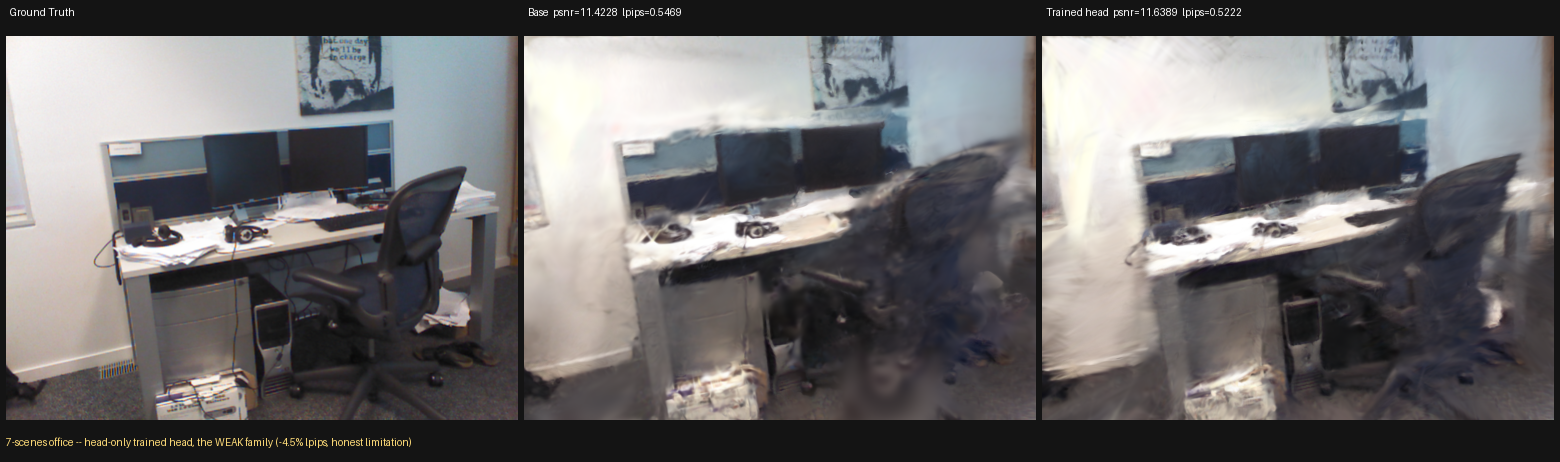
\includegraphics[width=0.92\linewidth]{fig/7scenes_office_f0.png}
  \caption{\textbf{Head-only adaptation, per family} (ground truth $|$ released
  checkpoint $|$ head-only fine-tuned), on held-out non-keyframe views. Rows:
  ETH3D \texttt{sofa\_1}, EuRoC \texttt{V1\_01}, TUM \texttt{fr1\_rpy},
  7-Scenes \texttt{office}. The first three are families where the recipe
  clearly helps; the last is the weak family
  ($+0.14\%$ to $-4.9\%$ LPIPS), included so the failure mode is visible rather
  than only tabulated. Because the encoder is bit-frozen, the difference
  between the second and third panel of each row is attributable to the
  Gaussian head alone.}
  \label{fig:headonly}
\end{figure*}

\subsection{Injection-time thinning}
\label{sec:exp:thin}
Across $12$ online cells spanning four families, six heads and eight scenes:
$10$ clear benefits, $2$ ties, $0$ harmful cells, worst cell $+0.16\%$ LPIPS.
The confidence-weighted allocation of \cref{eq:thin} is shipped as the default,
though we note honestly that confidence-weighted versus uniform allocation is
statistically a coin flip at this sample size (median $-0.06\%$, CI containing
zero); we ship it because it is never much worse and it is the configuration
all deployment comparisons were run with.

\paragraph{Dose--response.}
If the effect were something a training-time penalty could supply, thinning
should lose its benefit once the head already produces well-separated
opacities. We measured two thinning depths on heads whose opacity distributions
differ, obtaining $-21.0\%$ and $-15.8\%$ LPIPS: neither collapsed toward
zero. Together with the observation that the refiner un-saturates opacity
unaided (median $1.0\rightarrow0.26$), this supports the reading of
\cref{eq:thin} as an acceleration of a trajectory the optimiser already
follows, rather than as information the network was missing.

\subsection{The opacity mechanism}
\label{sec:exp:mech}
\Cref{tab:lum} reports the pre-registered test. Heads trained under synthetic
darkening correlate opacity \emph{negatively} with input luminance; heads
trained on real sensor data correlate \emph{positively}. All five families
land on the predicted sign, with magnitudes clustering tightly.

\begin{table}[t]
\centering\small
\begin{tabular}{@{}llr@{}}
\toprule
Head & Training data & $\rho(\alpha,\text{luminance})$ \\
\midrule
photospatial & Replica + synthetic darkening & $-0.316$ \\
mixed        & Replica + synthetic darkening & $-0.279$ \\
TUM          & real sensor                   & $+0.303$ \\
ETH3D        & real sensor                   & $+0.392$ \\
EuRoC        & real sensor                   & $+0.304$ \\
\bottomrule
\end{tabular}
\caption{Pre-registered opposite-sign prediction, confirmed on $5/5$ families.
Both signs were registered before any number was computed.}
\label{tab:lum}
\end{table}

\subsection{Rendering: Replica, all eight scenes}
\label{sec:exp:replica}
\Cref{tab:replica} is the load-bearing rendering comparison: monocular against
monocular, on the benchmark this literature actually uses for rendering.

\begin{table}[t]
\centering\small
\setlength{\tabcolsep}{3.5pt}
\begin{tabular}{@{}lcccc@{}}
\toprule
\multirow{2}{*}{Scene} & \multicolumn{2}{c}{Ours} & \multicolumn{2}{c}{Photo-SLAM} \\
\cmidrule(lr){2-3}\cmidrule(lr){4-5}
 & PSNR\up & LPIPS\dn & PSNR\up & LPIPS\dn \\
\midrule
office0 & \best{26.30} & \best{0.104} & 22.23 & 0.209 \\
office1 & \best{22.08} & \best{0.115} & 17.80 & 0.185 \\
office2 & \best{20.97} & 0.151 & 20.24 & \best{0.129} \\
office3 & \best{20.18} & \best{0.144} & 19.36 & 0.155 \\
office4 & \best{23.65} & 0.156 & 16.46 & \best{0.125} \\
room0   & \best{25.44} & \best{0.110} & 17.92 & 0.152 \\
room1   & \best{21.91} & \best{0.140} & 21.88 & 0.175 \\
room2   & \best{23.62} & 0.160 & 20.75 & \best{0.116} \\
\midrule
Mean    & \best{23.02} & \best{0.135} & 19.58 & 0.156 \\
\bottomrule
\end{tabular}
\caption{Replica, monocular, one protocol. We lead PSNR on $8/8$ but LPIPS on
only $5/8$. A three-scene subset (office0, office1, room0) would have reported
$+5.29$\dB{}; all eight give $+3.44$\dB{}, and three scenes are effectively
ties ($+0.03$, $+0.73$, $+0.81$).}
\label{tab:replica}
\end{table}

\begin{figure*}[t]
  \centering
  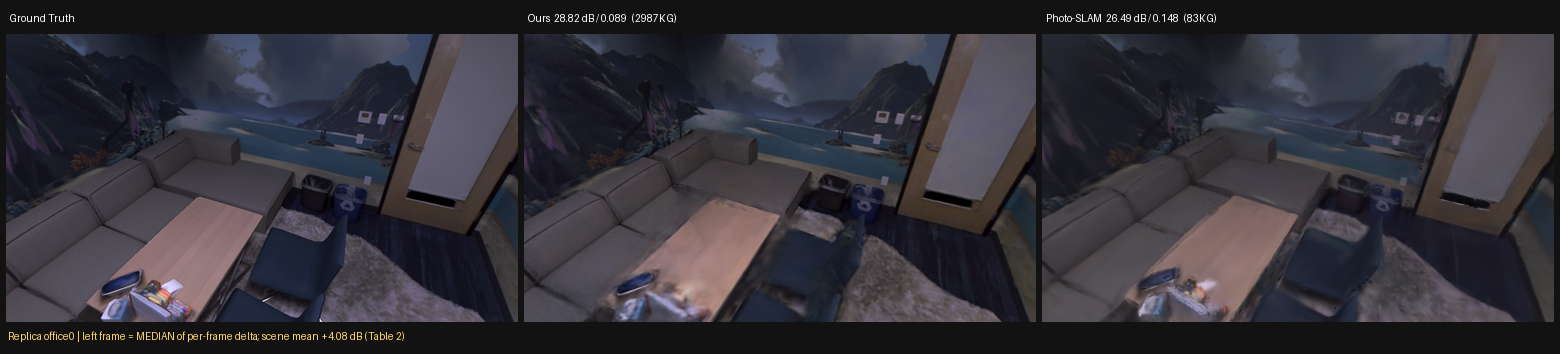
\includegraphics[width=0.92\linewidth]{fig/cmp_replica_office0_f1.png}
  \caption{\textbf{Replica office0, one protocol.} A second baseline comparison
  under the identical protocol used for \cref{fig:teaser}, on a scene where our
  margin is closer to the Replica mean ($+4.08$\dB{} versus the $+3.44$\dB{}
  eight-scene mean) rather than at the top of the range.}
  \label{fig:office0}
\end{figure*}

\paragraph{Means hide the distribution.}
Scoring $24$ probe frames per scene individually, the per-frame $\Delta$PSNR
median is $+8.01$ on room0 and $+3.62$ on office0, but $\mathbf{-1.84}$ on
office2 --- a scene whose \emph{mean} says we lead by $+0.73$\dB{}. Our nominal
win there comes from a minority of frames, not from being typically better.
Even on room0, Photo-SLAM wins some frames ($\min\Delta = -4.77$). Qualitative
figures in this paper are therefore selected at the median of the per-frame
delta, not by eye.

\subsection{Rendering: TUM, and the budget question}
\label{sec:exp:tum}
\Cref{tab:tum} reports TUM \texttt{fr1\_desk}, the only TUM sequence where all
three rendering systems track successfully. At \emph{matched wall clock} ---
our $300$\,s polish against MonoGS's $339$\,s refinement --- PSNR ties and
MonoGS wins LPIPS. Only with $3.5\times$ their budget do we lead both. The
honest statement is that MonoGS has better perceptual quality at equal compute
and we can buy past it with more, not that our deficit was a budget artefact.

\begin{table}[t]
\centering\small
\setlength{\tabcolsep}{4pt}
\begin{tabular}{@{}lccrr@{}}
\toprule
System & PSNR\up & LPIPS\dn & Gauss. & Budget \\
\midrule
Ours ($300$\,s)   & 13.95 & 0.411 & 2.40M & $\sim$1.4k st. \\
MonoGS ($339$\,s) & 13.87 & \best{0.398} & \best{23K} & 26k it. \\
Photo-SLAM        & 10.73 & 0.558 & 36K & to shutdown \\
\midrule
Ours ($1200$\,s)  & \best{14.61} & \best{0.379} & 2.40M & $\sim$4.4k st. \\
\bottomrule
\end{tabular}
\caption{TUM \texttt{fr1\_desk}. This comparison cannot be extended to further
TUM sequences: MonoGS's monocular tracking diverges on them
(\cref{tab:ate}), and scoring rendering against a diverged map would measure
tracking failure rather than rendering quality.}
\label{tab:tum}
\end{table}

\subsection{Trajectory accuracy}
\label{sec:exp:ate}
\Cref{tab:ate} completes the trajectory picture. The finding is
\emph{robustness}, not precision: Photo-SLAM and MonoGS each diverge on
several sequences ($0.30$--$0.84$\,m, i.e.\ failure rather than error), which
is what dominates their means, while on sequences they do track Photo-SLAM is
frequently the most accurate. We stress that our parity with MASt3R-SLAM
(4--4--1, noise) is \emph{expected and not a contribution}: the tracking
front-end is inherited unchanged, which \cref{tab:ate} verifies externally
rather than by assertion.

\begin{table}[t]
\centering\small
\setlength{\tabcolsep}{3pt}
\begin{tabular}{@{}lrrrrr@{}}
\toprule
Seq. & Ours & MASt3R & VGGT & Photo & MonoGS \\
\midrule
360   & 0.042 & 0.048 & 0.050 & \best{0.035} & 0.177 \\
desk  & 0.017 & 0.016 & 0.025 & \best{0.015} & 0.036 \\
desk2 & \best{0.028} & 0.024 & 0.029 & 0.438 & 0.844 \\
floor & 0.027 & 0.025 & 0.099 & \best{0.013} & 0.539 \\
plant & \best{0.015} & 0.020 & 0.025 & 0.046 & 0.071 \\
room  & \best{0.059} & 0.061 & 0.064 & 0.510 & 0.791 \\
rpy   & 0.022 & 0.023 & 0.026 & 0.057 & \best{0.041} \\
teddy & 0.048 & 0.045 & \best{0.036} & 0.305 & 0.123 \\
xyz   & 0.009 & 0.009 & 0.014 & \best{0.010} & 0.017 \\
\midrule
Mean  & \best{0.030} & 0.030 & 0.041 & 0.161 & 0.293 \\
\bottomrule
\end{tabular}
\caption{ATE RMSE (m), TUM freiburg1, all nine sequences and all five systems.
Photo-SLAM is non-deterministic (ORB-SLAM3 is multi-threaded): \texttt{desk}
gave $0.0174$ and $0.0149$ on two runs, so its single-run figures carry
run-to-run variance.}
\label{tab:ate}
\end{table}

\subsection{Front-end geometry is not the lever}
\label{sec:exp:frontend}
\Cref{tab:ate} raises an obvious design question, and we answer it by
measurement rather than argument. The per-keyframe scale jitter behind the
visible seams in our maps is a two-view artefact: each cluster's scale is
decided by one independent forward, and neighbouring clusters are decided by
different ones. Would our contributions therefore be better carried by a joint
many-view front-end such as VGGT-SLAM~\cite{maggio2025vggtslam}? We ran that
question in four stages. It is a negative result, and it has a mechanism.

\paragraph{Joint context removes the jitter; a better backbone does not.}
We measure adjacent-view depth-scale disagreement against RGB-D depth in a
gauge-free form --- per window, the spread of the scale each view implies,
normalised so that no global gauge enters. \Cref{tab:scale} is the resulting
$2\times2$. The \emph{same} VGGT~\cite{wang2025vggt} weights on the
\emph{same} pairs are $2.0\times$ \emph{worse} than the incumbent two-view
backbone when run pairwise, and $6.4\times$ better when sixteen views are
coupled in one forward. Changing the architecture makes it worse; changing the
context makes it better. The gain is attributable to multi-view context, not
to a stronger prior --- and our deployment regime is the causal two-view one,
which is precisely VGGT's weakest mode. A drop-in backbone swap would buy the
$10.82\%$ row, not the $1.68\%$ one.

\paragraph{Averaging cannot substitute for coupling.}
The cheap version of the same idea needs no new backbone: at keyframe
creation, predict the new view against $m$ well-overlapping partners,
scale-align the $m$ depth maps and average. Measured over
$m\in\{1,2,4,8\}$ this saturates at $5.16\%\rightarrow3.06\%$ --- a factor of
two above what coupling reaches, at $m$ forwards per keyframe. Independent
draws cancel; a gauge does not.

\paragraph{The referee is right, and the picture gets worse.}
We then used one joint sixteen-view forward over all of a map's keyframes as
an external scale referee, taking the per-cluster scalar corrections it
implies --- normalised to median one, so the map's global scale is untouched
--- and applying them to the baked map. Absolute per-keyframe scale error
against the sensor improves $6.35\times$ ($6.48\%\rightarrow1.02\%$ on
\texttt{fr1\_desk}; $2.2$--$2.3\times$ on \texttt{360} and \texttt{room}),
and held-out PSNR \emph{falls} from $12.35$ to $11.50$\dB{} with LPIPS rising
$0.507\rightarrow0.523$. A $300$\,s polish does not recover it
($13.81\rightarrow13.08$). The obvious escape --- that the referee is
incompetent on SLAM keyframes, which are selected to be as dissimilar as
possible, unlike the consecutive views it was validated on --- was audited by
scoring map and referee against the sensor on exactly those keyframes: the
referee is $2.2$--$6.4\times$ the more accurate of the two. The referee is
right and the rendering still degrades.

\paragraph{The same conflict inside the refiner.}
Supplying the corrections as a \emph{prior} rather than an edit, with keyframe
translations freed so the photometric term is able to disagree, is monotone in
the prior weight and monotone the wrong way: PSNR $13.74\rightarrow13.38$ and
LPIPS $0.449\rightarrow0.456$ as the weight goes $0.05\rightarrow0.5$, and
even at the largest weight the fitted scale spread is $2.6\%$ against the
referee's $8.0\%$. The photometric term is still winning the argument, and
forcing it further is what the previous paragraph already measured as harmful.

\paragraph{What this establishes.}
In a trajectory-anchored map, rendered quality is not governed by absolute
geometric accuracy. SLAM fits each keyframe's pose to that keyframe's own
biased pointmap, so much of the per-cluster scale error is \emph{common-mode}
with the pose. The photometric evaluation is structurally blind to common-mode
depth error at these baselines --- $4.5\%$ of depth is $0.66$\,px at
\texttt{fr1\_desk}'s $0.057$\,m median keyframe baseline --- but it is not
blind to two overlapping clusters disagreeing about where a surface is, and
correcting a cluster alone converts an absorbed error into exactly that
differential displacement. The two objectives do not even agree in rank: the
photometric fit asks for a $0.8\%$ per-keyframe correction where the sensor
says the map is $6.5\%$ wrong, with Spearman $+0.06$ between them. Every
post-hoc per-cluster geometric correction is therefore closed, and the jitter
can only be removed where poses and per-keyframe scales are solved
\emph{together} --- in the back-end, which is a different system rather than a
component swap. This is why our front-end is inherited unchanged, and it is
also why a joint front-end is not a shortcut to our open problems: VGGT-SLAM
already costs $9{,}436$\,MiB (\cref{sec:exp:cost}) while producing no
renderable map at all.

\begin{table}[t]
\centering\small
\setlength{\tabcolsep}{5pt}
\begin{tabular}{@{}llrr@{}}
\toprule
Predictor & Context & Views & Disagreement \dn \\
\midrule
Splatt3R (deployed) & pairwise & 2 & $5.35\%$ \\
VGGT~\cite{wang2025vggt} & pairwise & 2 & $10.82\%$ \\
VGGT~\cite{wang2025vggt} & joint & 16 & \best{$1.68\%$} \\
\midrule
\multicolumn{4}{@{}l}{\emph{disjoint-window replication}} \\
Splatt3R & pairwise & 2 & $4.92\%$ \\
VGGT & joint & \phantom{0}8 & \best{$1.53\%$} \\
\bottomrule
\end{tabular}
\caption{Adjacent-view depth-scale disagreement, gauge-free, TUM freiburg1,
pooled over seven sequences ($84$ windows above the rule, $33$ disjoint
windows below it). Windows in the primary arm overlap by $80$--$97\%$, so the
result is replicated on eight-view windows tiled by exactly one span; the
replication is $7/7$ sequences, paired Wilcoxon $p=8.6\times10^{-8}$. VGGT's
$1.68\%$ sits at or below the RGB-D sensor's own view-dependent bias floor, so
it is a lower bound on how far coupling goes.}
\label{tab:scale}
\end{table}

\subsection{Refinement ablations}
\label{sec:exp:refiner}
\Cref{tab:refiner} isolates the components of \cref{sec:method:refiner}. The
refiner's own contribution, measured with the base checkpoint on both arms so
that only the refiner toggles, is large and consistent across families:
$+8.69$\dB{} on ETH3D, $+4.62$\dB{} on Replica, $+3.52$\dB{} on TUM and
$+1.00$\dB{} on EuRoC. This is not a marginal add-on next to head-only
training --- on ETH3D it exceeds it --- and the two levers stack rather than
compete.

\begin{table}[t]
\centering\small
\setlength{\tabcolsep}{4pt}
\begin{tabular}{@{}lrl@{}}
\toprule
Ablation & $\Delta$PSNR & Note \\
\midrule
Refiner on, ETH3D   & $+8.69$ & 300\,s polish \\
Refiner on, Replica & $+4.62$ & \\
Refiner on, TUM     & $+3.52$ & \\
Refiner on, EuRoC   & $+1.00$ & \\
\midrule
Causal replay, 120 it. & $+1.21$ & strict real time \\
Second GPU, unthrottled & $+2.15$ & latency $+1\%$ \\
\midrule
Uniform vs.\ recency & $+0.34$ & held-out mean \\
Voxel dedup, 10\,mm & $-0.53$ & $-27.6\%$ map size \\
\bottomrule
\end{tabular}
\caption{Refinement ablations. ATE is unchanged in every row
($0.016975$ vs.\ a $0.0170$ baseline in the deterministic configuration): the
map is strictly downstream of tracking, and the pre-registered failure
condition ``ATE moves at all'' never fired. Freezing the Gaussian centres was
separately measured optimal at both the online ($\sim$300-step) and offline
(3000-step) budgets. The dedup row is included as a negative: it is a map-size
control that costs quality when it fires without a recovery budget, not a
quality feature.}
\label{tab:refiner}
\end{table}

\subsection{Online delivery across dataset families}
\label{sec:exp:online}
The offline ablations above use a controlled polish budget. We therefore also
ran the actual deployed path: a per-family head, causal SLAM, GUI enabled, and
the refiner on the second GPU. \Cref{tab:online} reports the paired map
quality; the refiner never receives or writes a pose correction.

\begin{table}[t]
\centering\small
\setlength{\tabcolsep}{2.7pt}
\begin{tabular}{@{}llrrrr@{}}
\toprule
Family & Sequence & Bake P & Refine P & $\Delta$P & $\Delta$L \\
\midrule
TUM & desk & 12.42 & 13.75 & +1.33 & $-7.5\%$ \\
TUM & room & 11.15 & 11.45 & +0.30 & $+11.1\%$ \\
TUM & 360 & 12.00 & 12.14 & +0.14 & $+20.6\%$ \\
7-Scenes & chess & 13.44 & 13.79 & +0.35 & $-4.8\%$ \\
7-Scenes & office & 11.64 & 11.74 & +0.10 & $-1.6\%$ \\
7-Scenes & pumpkin & 14.15 & 14.91 & +0.77 & $-4.1\%$ \\
EuRoC & MH\_01 & 10.17 & 11.67 & +1.50 & $-4.1\%$ \\
EuRoC & V1\_01 & 12.06 & 12.69 & +0.63 & $-13.0\%$ \\
ETH3D & plant\_1 & 20.42 & 22.22 & +1.80 & $-7.4\%$ \\
\bottomrule
\end{tabular}
\caption{Actual GUI-on, dual-GPU online delivery. P is PSNR in dB and L is
LPIPS; $\Delta L$ is relative, so negative is better. Seven of nine cells
improve LPIPS. TUM room and 360 gain a little PSNR but lose perceptual quality
under the in-sequence budget, exposing supervision starvation on their large
maps rather than a universal refiner improvement. ETH3D \texttt{cables\_1} is
omitted because its $0.5$-m scene and $0.1165$-m ATE make held-out rendering
alignment-dominated. The reported online values are from the pre-polish
delivery pass; the longer polish diagnostic is separated below.}
\label{tab:online}
\end{table}

The deployment cost is measurable rather than merely architectural. Across
the nine online runs, the second-GPU refiner costs approximately $7$--$10\%$
frame time with the GUI open. The head-only arm uses $19.8$--$39.6$~GB on
GPU0; enabling refinement adds $1$--$1.5$~GB on GPU0 and $2.8$--$14.0$~GB on
GPU1, with the largest observed combination $41.1$~GB plus $14.0$~GB on the
two cards. These measurements define the practical operating envelope: the
refiner is deployable, but memory remains proportional to the assembled map.

\paragraph{Budget, not a simple position prior.}
The online TUM room/360 degradation initially suggested a position-learning
rate failure. That explanation came from an offline proxy and did not survive
the causal loop. The deployed sequences supplied only $104/114/190$ refiner
steps for desk/360/room maps, whereas a post-sequence polish producing
$1581/3821/1856$ steps improved PSNR by $+1.97/+2.30/+2.22$~dB and LPIPS by
$-22.0/-8.3/-15.9\%$, respectively. We therefore reverted the offline
position-freezing and band-limit defaults rather than presenting them as a
universal online fix. This is a concrete example of why causal delivery and
offline polish are separate experimental regimes.

\subsection{System cost}
\label{sec:exp:cost}
On TUM \texttt{fr1\_desk}, one GPU, one sampler for all systems: ours
$70$\,s wall clock at $21{,}035$\,MiB peak; Photo-SLAM $28$\,s at
$1{,}286$\,MiB; MonoGS $555$\,s at $2{,}389$\,MiB; VGGT-SLAM $24$\,s at
$9{,}436$\,MiB. Our peak memory is $16\times$ Photo-SLAM's and $8.8\times$
MonoGS's, and Photo-SLAM is $2.5\times$ faster end-to-end.
